\documentclass[12pt]{article}
\usepackage[top=2cm,bottom=2cm,left=2cm,right=2cm]{geometry} %define borders
\usepackage{url}
\usepackage{paralist}
\usepackage{xcolor,graphicx,wrapfig,mytikz}
%\usepackage[T1]{fontenc}

\usepackage[bookmarksnumbered,bookmarksopen,colorlinks,urlcolor=gray,linkcolor=blue,citecolor=blue]{hyperref}

\usepackage{basics}

\newcommand{\defemph}[1]{\textbf{#1}}
\newcommand{\enclcite}[1]{\cite{#1}}
\newcommand{\citeByNumber}[1]{\cite{#1}}

\newcommand{\LFI}{LFI}
\newcommand{\cn}[1]{\mathtt{#1}}
\newcommand{\pn}{LATIN}

\begin{document}

\author{Florian Rabe}
\title{MMT: A Foundation-Independent Approach to Formal Knowledge}
\date{\today}
\maketitle

\begin{abstract}
\mmt is a framework for representing declarative languages such as logics, type theories, set theories, etc..
It achieves a high level of generality by systematically avoiding a commitment to a particular syntax or semantics.
Instead, individual language features (e.g., $\lambda$-abstraction, conjunction, etc.) and syntax features (keywords, notations, etc.) are defined as separate, reusable modules, from which individual languages are assembled.
These modules can be declarative by specifying features as \mmt theories or programmatic by providing individual rules as plugins.

Despite this high degree of abstraction, it is possible to implement advanced algorithms generically at the \mmt level.
These include knowledge management algorithms (e.g, IDE, search, change management) as well as logical algorithms (e.g., parsing, type reconstruction, module system).
Thus, we can use \mmt to obtain strong implementations of declarative languages at extremely low cost.

Moreover, the focus on modularity and language-independence enables system integration, where \mmt can mediate the exchange of knowledge across different foundational systems and concrete syntaxes.
\end{abstract}

\section{Motivation}\label{sec:motiv}

Methods based on formal knowledge pay off almost exclusively at large scales due to the high level of theoretical understanding and practical investment that they require from both developers and users.
But for the same reason, it is difficult for individual approaches to reach those large scales.
Today's successful projects such as the Mizar Mathematical Library \cite{mizar}
%verification of the L4 microkernel \cite{l4verified}
or the formal proof of the Kepler conjecture \cite{flyspeck}
are built on double-digit person years of investment.

Therefore, the last few decades have seen increasing specialization into isolated, mutually incompatible systems and incompatible overlapping libraries of formal knowledge.
Moreover, during that time the advances in computer and internet technology have dramatically changed our expectations regarding scalability.
Many requirements have become critical that are not anticipated in the designs of formal systems such as collaboration, system interoperability, and modularity.
Three central design choices have proved problematic:

{\bf Fixed Foundations}
Virtually all current systems are based on a fixed foundation, i.e., a fixed logic in which all formalizations in that system are stated.
While the vast majority of classical mathematics has been formulated in axiomatic set theory, alternative foundations such as higher-order logic or constructive type theory have become important in computer-supported approaches.
Today almost all systems use foundations that are different from each other and different from classical set theory, and all attempts to find the ``mother of all logical systems'' (and convince others to use it) have failed, e.g., the qed project \cite{qed}.
This is all the more frustrating because these incompatibilities are often irrelevant for high-level formalization goals.
  
{\bf Homogeneity}
Classical mathematics uses the heterogeneous method, going back to the works by Bourbaki \cite{bourbakiunivers}, which focuses on defining \emph{theories} and stating every result in the smallest possible theory.
This allows using \emph{theory morphisms} to move results between theories in a truth-preserving way \cite{littletheories}.
Consequently, mathematics is usually carried out in highly abstracted settings where the foundational details are hidden.
Yet, virtually all formalizations in current systems are based on the homogeneous method, which uses only conservative extensions (e.g., definitions, theorems) of the fixed foundation to model mathematical knowledge.
Therefore, formalizations inherently depend on the fixed foundation.
%The combination of fixed foundation and homogeneous method means that a lot of -- expensive -- formalization work is needed just to build the mathematical setting of interest (e.g., the real numbers) as a conservative extension of the fixed foundation.
%However, the resulting formalizations are actually less valuable: It becomes virtually impossible to move them between foundations.
%Therefore, almost all current systems are mutually incompatible, with only a few hand-crafted translations between them (e.g., \cite{hol_coq,isahol_isazf}).

{\bf Local Scale} Mathematical research and applications are distributed globally, and mathematical knowledge is highly interlinked by explicit and implicit references.
Therefore, a computer-supported management system should support global interlinking, and management algorithms have to scale up to large (global) data sets.
Yet, virtually all current systems operate under the implicit assumption that all knowledge is locally available and loaded into main memory.
In fact, because these systems have initially focused on soundness and efficiency at small scales, large scale knowledge management has proved very difficult to add as an afterthought, often prohibitively so.
%many are designed in such a way that every run of the system verifies not only the theorem at hand but every single theorem leading up to it.
\medskip

However, developers' resources are stretched thin already by developing (and maintaining) their system at all.
Therefore, the gradual migration towards new designs that overcome these problems is extremely difficult.

The {\mmt} language and system have been designed from scratch to provide a uniform solution to the above three problems: a globally scalable Module system for Mathematical Theories.
It abstracts from and mediates between different foundations and maximizes the reuse of concepts, tools, and formalizations.
Thus, it provides a theoretical and practical foundation for formal knowledge in the large.

\section{The \mmt Language}

\mmt is systematically \textbf{foundation-independent}.
It separates large scale concerns, which are addressed generically by {\mmt}, and small scale concerns, which are addressed by individual foundational languages.
Thus, foundation-specific development can focus on the logical core of the foundation instead of spending resources on ad hoc large scale support.
Dually, large scale support can be developed generically (and often more easily) at the {\mmt} level.

\mmt integrates successful features of existing paradigms
\begin{compactitem}
\item reuse along theory morphisms from the ``little theories'' approach \cite{littletheories},
\item the structured theories from algebraic specification languages like \cite{asl},
\item categories of theories and logics from model theoretical logical frameworks like institutions \cite{institutions},
\item the logics-as-theories representation from proof theoretical logical frameworks like LF \cite{lf},
%\item declarations of constants and named realizations from type theory,
\item the Curry-Howard correspondence from type/proof theory \cite{curry,howard},
\item URIs as logical namespace identifiers from {\openmath} \cite{openmath},
\item standardized XML-based concrete syntax from web-oriented representation languages like {\omdoc} \cite{omdoc},
\end{compactitem}
and makes them available in a single, coherent representational system for the first time.
The combination of these features is reduced to \textbf{a small set of carefully chosen, orthogonal primitives} in order to obtain a simple and extensible language design.
%In particular, {\mmt} coherently realizes two goals that are often mutually exclusive in knowledge representation languages:
%\begin{inparaenum}[(i)]
% \item the automation potential offered by machine-understandable representations, as pursued for example in proof assistants
% \item the universal applicability offered by a generic meta-language, as pursued in XML-based content markup languages.
%\end{inparaenum}
%Being a foundationally unconstrained language with a precise semantics

The central concept of \mmt is that of a \textbf{theory}, which is a named list of declarations.
Most importantly, the declaration of a \textbf{constant} introduces a new name possibly with additional attributes such as type, definiens, or notation.
Relative to a theory, \textbf{objects} are formed as syntax trees with binding.

These three concepts are sufficient to naturally represent virtually all formal languages.
\begin{compactitem}
\item All languages such as are represented uniformly as {\mmt} theories.
This includes foundations, logical frameworks, logics and type theories, signatures and theories, set theories.
\item All operators and symbols of a language are represented as \mmt constants.
This includes the sort, constant, function, and predicate symbols of logics, the base type, type operators, and term constructors of type theories, the concepts, relations, and individuals of ontologies, as well as -- via the Curry-Howard correspondence -- the judgments, inference rules, axioms, and theorems of calculi.
\item All composed expressions are represented as objects.
This includes formulas, derivations and proofs, terms, types, kinds, and universes, etc.
\end{compactitem}

All {\mmt} theories are related via \textbf{theory morphisms}, which are used to uniformly describe representation theorems between theories.
These include translations, functorial representations, implementations, and models.
They are also used as the semantics of \textbf{import} declarations within theories, which uniformly represent all aspects of building theories modularly.
These include inheritance and instantiation.

\begin{wrapfigure}r{6cm}
\vspace{-1em}
\begin{tikzpicture}[xscale=.95]
\node (A) at (0,3)  {$\cn{LF}$};
\node (A') at (2,3)  {$\cn{LF}+X$};
\node (C) at (-1,1.5)   {$\cn{FOL}$};
\node (C') at (1,1.5) {$\cn{HOL}$};
\node (E) at (-3,0) {$\cn{Monoid}$};
\node (E') at (1,0)  {$\cn{Ring}$};
\draw[dotted,arrow](A) -- (C);
\draw[dotted,arrow](A) -- (C');
\draw[dotted,arrow](C) -- (E);
\draw[dotted,arrow](C) -- (E');
\draw[dashed,arrow](A) --node[above] {$m$} (A');
\draw[arrow](C) --node[above] {$m'$} (C');
\draw[dashed,arrow](E) to[out=-30,in=-150] node[above] {$\cn{add}$} (E');
\draw[dashed,arrow](E) to[out=30,in=150] node[below] {$\cn{mult}$} (E');
\end{tikzpicture}
\end{wrapfigure}

A key innovation of {\mmt} is the \textbf{meta-theory} import between theories.
Let us write $M/T$ to express that we work in the object language $T$ using the meta-language $M$.
For example, most of mathematics is carried out in $\cn{FOL}/\cn{ZFC}$, i.e., first-order logic is the meta-language, in which set theory is defined.
$\cn{FOL}$ itself might be defined in a logical framework such as $LF$~\cite{lf}, and within $ZFC$, we can define the language of natural numbers, which yields $\cn{LF}/\cn{FOL}/\cn{ZFC}/\cn{Nat}$.

In {\mmt}, all of these languages are represented as theories, each of which may be reused as the meta-theory of another one.
Crucially, the meta-theory indicates both to humans and to machines how a theory is to be understood.
For example, interpretations of $\cn{ZFC}$ must understand $\cn{FOL}$, and the typing relation of $\cn{FOL}$ is inherited from $\cn{LF}$.
The diagram in the category of \mmt theories gives an example, where dotted arrows denote the meta-theory relations, solid arrows are language translations, and dashed arrows are imports.
$\cn{LF}+X$ represents any extension of LF with additional features.

The module system is tightly coupled with the use of URIs as identifiers -- a design goal that imposes so subtle constraints that it is difficult to retrofit to a non-modular system.
In {\mmt}, all knowledge items, including the virtual ones that only arise by reuse along morphisms have canonical, globally unique URIs.
These are tripartite URIs $ns?mod?sym$ formed from a namespace URI $ns$, a module name $mod$, and a qualified symbol name $sym$.

To facilitate distributing {\mmt} content, all {\mmt} URIs are logical identifiers, and their physical locations (URLs) remain transparent to the {\mmt} language: the relation between logical URIs and physical URL is delegated to an extra-linguistic catalog.
\medskip

We can see {\mmt} as the last step in a historical progression towards more abstract frameworks as indicated below.
In traditional mathematics, domain knowledge is expressed directly in ad hoc formal notation.
Starting in the 20th century, logic provided a formal syntax and semantics for expressing this knowledge.
Starting in the 1970s, logical frameworks provided an additional level of abstraction, at which individuals logics could be treated uniformly.
Now {\mmt} provides a meta-level, at which even different logical frameworks can be represented.
Therefore, {\mmt} is robust against future language developments: We can develop new logical frameworks and use them to define new logics without any change to the {\mmt} infrastructure.
{\mmt} guarantees the theoretical and practical reusability of developments when migrating to these new languages.

\begin{center}
\begin{tabular}{|l|l|l|l|}
\hline
Mathematics      & Logic            & Logical Frameworks & Foundation-Independence \\
\hline
%natural language & natural language & natural language & natural language \\
                 &                  &                  & {\mmt}\\
                 &                  & logical framework & logical framework\\
                 & logic            & logic            & logic\\
domain knowledge & domain knowledge & domain knowledge & domain knowledge \\
\hline
\end{tabular}
\end{center}

%%%%%%%%%%%%%%%%%%%%%%%%%%%%%%%%%%%%%%%%%%%%%%%%%%%%%%%%%%%
\section{The \mmt System}\label{sec:mmtsys}

Exploiting the small number of primitives in {\mmt}, the {\mmt} API provides a comprehensive, scalable implementation of {\mmt} itself and of {\mmt}-based knowledge management services. All algorithms are implemented generically, and all logic-specific aspects are relegated to thin plugin interfaces.

It is written in the functional and object-oriented language Scala \cite{scala}. Scala is fully compatible with Java so that API plugins and programs using the API can be written in any combination of Scala and Java.
The API depends on only one external library -- the lean web server tiscaf \cite{tiscaf}.
Excluding plugins and libraries, it comprises over $20000$ lines of Scala code compiling into about $3000$ Java \texttt{class} files totaling about $5$ MB of platform-independent bytecode.
Sources, binaries, API documentation, and user manual are available at \url{http://trac.kwarc.info/MMT}.

\paragraph{Knowledge Management Services}
The {\mmt} API provides a suite of coherently integrated MKM services.

{\mmt} content is organized in {\mmt} archives \citeByNumber{2f}, a light-weight project abstraction that integrates the representational dimensions of source files, content structure, narrative document structure, presentation, and semantic web-ready relational indices.

Source files form the original representation, which is usually subject to change by human editing.
When importing sources into {\mmt}, it splits them into content and narrative structure, which are given concretely as XML markup based on the {\omdoc} language \cite{omdoc}.
The former the semantically relevant information such as definitions and axioms; the latter contains the various possible linearized narrative structure, which can include connecting text and cross-references.

Both are used to generate presentation, which is dual to source in that it is tailored towards reading rather than editing, e.g., by using HTML with embedded presentation MathML \cite{mathml}.
The generation of presentation employs a notation language based on \citeByNumber{2b}.
The notations are grouped into styles, and the {\mmt} a presentation engine serializes any {\mmt} into arbitrary output formats according to the chosen style.

The crucial feature of {\mmt} archives is that all representational dimensions share the {\mmt} URIs, which permits concise cross-referencing.
For example, {\mmt} URIs are used for fine-granular parallel markup, i.e., every nodes in the presentation tree point to the corresponding content node, which in turn points to the corresponding point in the source file.

The relational index uses the {\mmt} URIs as the individuals in an {\mmt} ontology.
A query language and evaluation engine \citeByNumber{2h} integrates semantic web-style relational queries with hierarchical queries based on the content structure and unification-based queries provided by \cite{mathwebsearch,IK:flatsearch:12}.

Moreover, the canonical URI feature centrally a change management infrastructure \citeByNumber{2g}: They permit the fine-granular representation of changes to {\mmt} content.
The {\mmt} change management engine detects and propagates such changes.

\paragraph{User and System Interfaces}
The API can be run as an application, in which case it responds with a shell that interacts via standard input/output.
The shell is scriptable in the sense that sequences of commands can be read from files, which also provides an easy way for users to initialize and configure the system.

The main frontend is given by an HTTP server.
For machine interaction, it exposes all API functionality including services such as querying and presentation.
For human interaction, it offers an interactive web browser based on HTML+presentation MathML generated by the presentation engine.
Based on the JOBAD JavaScript library \citeByNumber{2c} and {\mmt}-specific JavaScript bindings, user interaction is handled via JavaScript and Ajax.
The parallel markup between presentation, content, and source permits sophisticated interface functions, e.g., folding subexpressions, hiding/showing inferred types, implicit arguments, and redundant brackets, retrieving the definition of a symbol, or dynamically inferring the type of a subexpression.
\medskip

The {\mmt} API implements a catalog that maps {\mmt} URIs to their physical locations.
The catalog also acts as an abstraction over various backends that physically store {\mmt} archives.
{\mmt} knowledge items are retrieved from these backends and loaded into memory transparently when needed.
Thus, memory constraints are hidden from high-level knowledge management services and users.

Supported backends are file systems, SVN working copies and SVN repositories, and  databases \cite{tntbase}.
In particular, the latter also supports {\mmt}-specific indexing and querying functions \citeByNumber{2d}, which permit, e.g., the efficient retrieval of the dependency closure of an {\mmt} knowledge item.
The combination of {\mmt} module system and {\mmt}-aware \citeByNumber{2e} received the MKM 2010 Best Paper Award.
%For example, the API acts as a {\tntbase} plugin to create {\mmt}-specific indices, which are used by an XQuery module to provide efficient {\mmt}-specific access methods. For example, 

\paragraph{Instantiating {\mmt} for Specific Languages}
{\mmt} archives are typically written in one fixed meta-theory (which is itself defined in a different archive).
For example, the LATIN archive is written using the meta-theory LF.
All API functionality is foundation-independent, but foundation-specific knowledge can be provided via one of two plugin interfaces: these provide information about the syntax or the semantics of the meta-theory.

Syntax plugins provide parsing methods that translate non-{\mmt} source syntax into {\mmt} content markup.
This is crucial to turn existing non-{\mmt} knowledge repositories into {\mmt} archives.
Such plugins have been developed for a varied list of languages: the ATP interface language TPTP \cite{tptp}, the ontology language OWL \cite{owl}, the Mizar language for formalized mathematics \cite{mizar}, and the Twelf implementation \cite{twelf} of LF.
In particular, these have been used to import the TPTP library and the Mizar library \cite{IKRU:mizar:11}.

Semantics plugins provide implementations of the typing relation, in which the {\mmt} language is parametric.
%Implementing these provides $M$-developers with a uniquely simple way of obtaining a scalable implementation of $M$, a methodology we call \emph{rapid prototyping for logics}.
Here the {\mmt} module system remains transparent for the plugin so that only the core type checking algorithms have to be implemented.
For example, the semantics plugin for LF comprises only 200 lines of code.
Moreover, for all logics defined in $\LFI$, no additional semantics plugin is required because their typing relations can be inherited from LF.

%\begin{figure}[ht]
%\includegraphics[width=\textwidth]{mmtserver-infer-type.jpg}
%\caption{{\mmt} Web Interface}\label{fig:mmtweb}
%\end{figure}

\section{Integrating Languages: The LATIN Atlas}\label{sec:atlas}

\begin{figure}[hbp]
\begin{center}
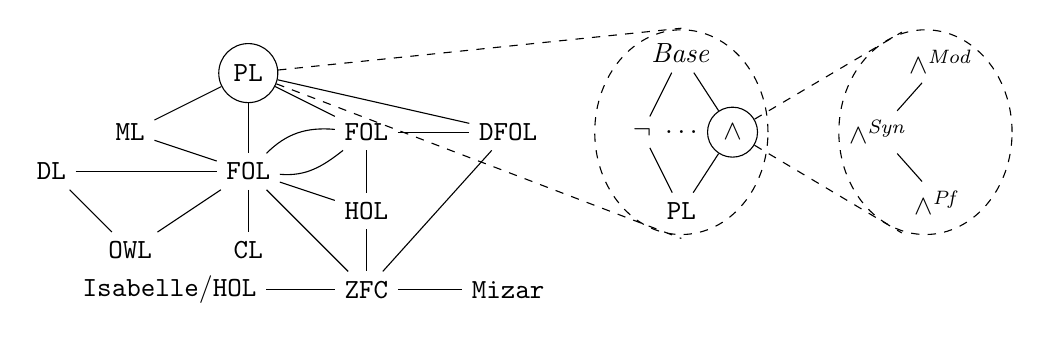
\begin{tikzpicture}
%The Logic Atlas
\node[circle,draw] (P)  at (4,4.25)   {$\cn{PL}$};
\node (M)  at (2.5,3.5) {$\cn{ML}$};
\node (S)  at (5.5,3.5) {$\cn{FOL}$};
\node (D)  at (7.3,3.5)   {$\cn{DFOL}$};
\node (F)  at (4,3)   {$\cn{FOL}$};
\node (C)  at (4,2)   {$\cn{CL}$};
\node (DL) at (1.5,3)   {$\cn{DL}$};
%\node (LL) at (1,3.5)   {$\cn{LL$};
\node (H)  at (5.5,2.5)   {$\cn{HOL}$};
\node (O)  at (2.5,2)   {$\cn{OWL}$};
\node (Mz) at (7.3,1.5)   {$\cn{Mizar}$};
\node (Z)  at (5.5,1.5)   {$\cn{ZFC}$};
\node (I)  at (3,1.5)   {$\cn{Isabelle/HOL}$};

\draw[\arrowtipmono-\arrowtip] (P) -- (F);
\draw[\arrowtipmono-\arrowtip] (P) -- (M);
\draw[\arrowtipmono-\arrowtip] (P) -- (S);
\draw[\arrowtipmono-\arrowtip] (P) -- (D);

\draw[-\arrowtip] (F)  -- (H);
\draw[-\arrowtip] (F)  -- (C);
\draw[-\arrowtip] (M)  -- (F);
\draw[-\arrowtip] (DL) -- (F);
\draw[-\arrowtip] (S)  -- (D);
\draw[-\arrowtip] (S)  -- (H);
\draw[-\arrowtip] (DL) -- (O);
\draw[-\arrowtip] (O)  -- (F);
\draw[-\arrowtip] (F) to[out=45,in=175] (S);
\draw[-\arrowtip] (S) to[out=218,in=-5]  (F);
\draw[-\arrowtip] (H)  -- (Z);
\draw[-\arrowtip] (D)  -- (Z);
\draw[-\arrowtip] (Z)  -- (Mz);
\draw[-\arrowtip] (I)  -- (Z);
\draw[\arrowtipmono-\arrowtip] (F) -- (Z);

%PL details with base, negation and conjunction
\node (B) at (9.5,4.5) {$\mathit{Base}$};
\node (N) at (9,3.5) {$\neg$};
\node (L) at (9.5,3.5) {$\ldots$};
\node[circle,draw] (A) at (10.15,3.5) {$\wedge$};
\node (PL) at (9.5,2.5) {$\cn{PL}$};
\draw[\arrowtipmono-\arrowtip] (B) -- (N);
\draw[\arrowtipmono-\arrowtip] (B) -- (A);
\draw[\arrowtipmono-\arrowtip] (N) -- (PL);
\draw[\arrowtipmono-\arrowtip] (A) -- (PL);
\draw[dashed] (9.5,3.5) ellipse (1.1cm and 1.3cm);
\draw[-,dashed] (P) -- (9.5,2.15);
\draw[-,dashed] (P) -- (9.5,4.82);

%Syn, Pf, Mod span for Conjunction
\node (AM) at (12.8,4.4)   {$\wedge^{\mathit{Mod}}$};
\node (AS) at (12,3.5) {$\wedge^{\mathit{Syn}}$};
\node (AP) at (12.8,2.6)   {$\wedge^{\mathit{Pf\,\,}}$};
\draw[\arrowtipmono-\arrowtip] (AS) -- (AP);
\draw[-\arrowtip] (AS) -- (AM);
\draw[dashed] (12.6,3.5) ellipse (1.1cm and 1.3cm);
\draw[-,dashed] (A) -- (12.3,4.77);
\draw[-,dashed] (A) -- (12.3,2.22);
\end{tikzpicture}
\end{center}
\caption{A Fragment of the LATIN Atlas}\label{fig:atlas}
\end{figure}

While some of these frameworks integrate the other side, such as the institution-based general logics developed in \cite{generallogics}, almost all of them lean towards either model or proof theory. Often these sides are divided not only by research questions but also by ``conflicting cultures and attitudes'', and ``attempts to bridge these two cultures are rare and rather timid'' (quoting an anonymous reviewer).

\enclcite{1a} makes one such attempt, trying to provide a balanced framework that integrates and subsumes both views on logic in a way that preserves and exploits their respective advantages.
This unified framework $\LFI$ picks one of the most successful frameworks from each side and combines them: institutions and LF.


The LATIN atlas is a library of representations of formal systems and translations in LF.
It includes not only logics but also type theories, set theories, and developments in category theory.
The logics are represented following the $\LFI$ framework, i.e., they are represented as spans of LF theories including syntax, proof theory, and model theory.
Similarly, the library includes various translations between these formal systems, many of which are logic translations in the sense of the $\LFI$ framework.

An overview of a fragment of the library is given in Fig.~\ref{fig:atlas}.
It shows a high-level logic graph on the left, then zooms into the modular definition of propositional logic in the middle, and on the right zooms in further to show the $\LFI$-style definition of conjunction as a triple of syntax, proof theory, and model theory.
\medskip

\enclcite{1a} first extends institutions with an abstract notion of proof theory arriving at a formal definition of \emph{logics}.
These logics are defined in the spirit of institutions, in particular retaining the abstraction from concrete syntax.
%Thus, they are very similar to the general logics of \cite{generallogics} and to the proof theoretic institutions of \cite{whatisalogicmossa,inswprfs}. We also discuss the use of meta-logics, which can be seen as a response to \cite{Tarlecki96moving}, where the use of a meta-institution is explored in general and the use of LF suggested in particular.
Then it defines a specific logic $\LFI$ based on LF that serves as a meta-logic.
The central idea is that a theory of $\LFI$ captures syntax, proof theory, and model theory of an object logic.
Similarly, $\LFI$-theory morphisms capture translations between object logics, including the translations of syntax, proof theory, and model theory.
$\LFI$ is defined in the spirit of LF, in particular retaining the focus on concrete syntax.
Consequently, judgments are represented as types and proofs as terms.
Moreover -- inspired by the ideas of Lawvere \cite{lawvere} -- models are represented as theory morphisms from the logical theory into a theory representing the foundation of mathematics.

Here the term ``foundation of mathematics'' refers to a fixed language in which mathematical objects are expressed.
While mathematicians usually do not explicate a foundation (often implicitly assuming a variant of first-order set theory as the foundation), the choice of foundation is more difficult in computational logic, where for example higher-order logic \cite{churchtypes} and the calculus of constructions \cite{calcconstructions} are often used instead.
By representing the foundation as a theory itself, $\LFI$ can formulate model theory without committing to a specific foundation.

Thus, $\LFI$ reconciles the type/proof and the set/model theoretical perspective: platonic, institution-based logics are expressed using the syntax of a formalist LF-based meta-logic.
\medskip

\begin{wrapfigure}{r}{3cm}
\vspace{-1em}
\begin{tikzpicture}	
\node (S) at (0,0) {$L^{Syn}$};
%\node (B) at (-2.5,0) {$Base$};
\node (P) at (1,1.3) {$L^{Pf}$};
\node (M) at (1,-1.3) {$L^{Mod}$};
\node (Z) at (1,-2.3) {$\mathcal{F}$};
\draw[-\arrowtip](S) --node[near end,left] {$L^{mod}$} (M);
\draw[right hook-\arrowtip](S) --node[near end,left] {$L^{pf}$} (P);
\draw[-\arrowtip](M) .. controls (.7,-1.8) .. node[left] {$M$} (Z);
\draw[\arrowtipmono-\arrowtip](Z) -- (M);
%\draw[\arrowtipmono-\arrowtip] (B) --node[above] {$L^{truth}$} (S);
\draw[-\arrowtip] (P) --node[right] {$L^{sound}$} (M);
\end{tikzpicture}
\vspace{-3em}
\end{wrapfigure}

In $\LFI$, logics are represented as theories and translations as theory morphisms in the category of LF-theories.
Logic representations formalize the syntax, proof theory, and model theory of a logic as separate theories as indicated on the right.
The syntax of a logic $L$ is represented as a theory $L^{Syn}$, which is then extended with the representation of proof rules to represent the proof theory as $L^{pf}$.
The model theory of the logic is represented as a theory $L^{Mod}$ as an extension of the representation $\mathcal{F}$ of a foundation of mathematics.
Then individual models are represented as theory morphisms $M$ into the foundation.
Moreover, we can represent soundness proofs as a morphism $L^{sound}$ from the proof theory to the model theory of $L$.
Similarly, logic translations are represented as triples of theory morphisms that formalize the translations of syntax, proof theory, and model theory.


All major research strands of the habilitation culminate in their relation to this library:
\begin{compactitem}
 \item The logics are defined within the $\LFI$ framework \citeByNumber{1a} where a formalist definition using LF induces a Platonist one using institutions.
 \item The formalist definitions are written using modular Twelf \citeByNumber{6}, which provides advanced authoring support.
 \item Twelf exports logic definitions using the modular representation language {\mmt} \citeByNumber{2a}.
 \item Twelf acts as a plugin to the {\mmt} system \citeByNumber{5}, which maintains the LATIN library as an {\mmt} archive and provides its knowledge management capabilities for it.
 \item The Platonist definitions become available as institutions to Hets via the integration of \citeByNumber{3d}.
\end{compactitem}
\medskip

The formalized logics include propositional, first-order, sorted first-order, common, higher-order, modal, description, and linear logics.
Their model theories can be represented in various foundations included Zermelo-Fraenkel set theory, Church's higher-order logic \cite{churchtypes}, or Mizar's formalized set theory \cite{mizar}.

Formalized logic translations include the relativization translations from modal, description, and sorted first-order logic to unsorted first-order logic,
%the interpretation of type theory in set theory,
the negative translation from classical to intuitionistic logic, and the translation from first to sorted first- and higher-order logic.

All representations systematically exploit modularity and form a single highly interconnected graph that currently consists of over 1000 little modules spread over about 200 files.
As a general principle, every logical principle is formalized in a separate module.
Such features are, for example, conjunction in propositional logic, the universal quantifier of first-order logic, the typed universal quantifier of sorted or higher-order logic, or the extensionality principle of higher-order logic.

Moreover, type theoretical features can be freely combined with logical features.
For example, the library includes modules for various type constructors such as the ones in the $\lambda$-cube or product and union types as well as base types like booleans or natural number.
Often multiple alternative formalizations are given (and related to each other), e.g., Curry- and Church-style typing, or Andrews and Prawitz-style higher-order logic.
\medskip

Thus, logics can be composed by adjoining the required features using the {\mmt} module system.
For example, the intuitionistic higher-order logic underlying the Isabelle system \cite{isabelle} can be obtained by combining the modules for Church-style typing, simple function types, a boolean type, implication, typed universal quantification, and typed equality, as well as corresponding modules for the semantics.
Similarly, new logics can be added easily by reusing some feature, adding a few additional features, and possibly relating the new features to the existing ones using translations.
In addition, some meta-results including logic translations and soundness proofs can be established feature-wise and composed modularly.

%It has now reached the critical size to grow steadily in the future.
%Since many reusable modules are already available, defining a new logic is often straightforward, at which point my work provides advanced tool support for that logic out of the box.

An overview of LATIN is given in \cite{CHKMR:latinabs:11}.
The atlas itself and the project report are available at \cite{project:latin}.
Particularly interesting representations include set theories \cite{IR:foundations:10}, model theory \cite{HR:folsound:10}, the logics underlying TPTP \cite{BRS:tptphol:08}.

Fig.~\ref{fig:mmtweb} shows a screenshot of the {\mmt} web server displaying a part of the LATIN archive (see Sect.~\ref{sec:atlas}), a collection of logic formalizations in $\LFI$.
This {\mmt} archive is written in Twelf syntax and uses the Twelf tool as a syntax plugin.
{\mmt} generates presentation, which can be browsed in the {\mmt} web server.

The selected declaration derives the rule $\frac{A,B\vdash C}{\vdash A\, imp\, (B\,imp\, C)}$ in the theory $\mathrm{IMP}$ of the implication connective $\mathrm{imp}$.
Via the JOBAD context menu, the user called type inference on the selected subobject, which resulted in a dialog displaying the dynamically inferred type.

The implementation of this feature uses server-side evaluation of {\mmt} queries.
JOBAD JavaScript picks up on the parallel markup annotations that carry the {\mmt} URIs of the presented content elements.
These are used to build an {\mmt} query that is evaluated on the server and results in the rendered inferred type, which is sent back to the client and displayed.
The query consists of multiple steps, which retrieve the corresponding mathematical object, extract the respective subobject (including its context), infer its type using the LF semantics plugin, and finally present it using the notation language.
\medskip

Due to the genericity of {\mmt} and the {\mmt} API, all this functionality can be made available to individual formal systems at minimal cost, a process we call \emph{rapid prototyping for formal systems}.
Given a syntax and a semantics plugin, {\mmt} provides the logical and the practical knowledge management infrastructure out of the box.


\section{Integrating Libraries:\\The Open Archive of Formalizations}

TPTP, Hets, Twelf, Mizar, HOL Light

On one side, \citeByNumber{3d} uses the Twelf \cite{twelf} implementation of LF as a representative of the implementations of proof theoretical logical frameworks.
Twelf uses LF as a universal logic in which other logics are represented, usually using higher-order abstract syntax \cite{hoas} and the Curry-Howard correspondence \cite{curry,howard}.

On the other side, \citeByNumber{3d} uses Hets \cite{hets}, an institution-independent software interface for heterogeneous (i.e., covering multiple logics)
specification and proof management.
Hets works relative to a graph of logics and logic translations, which connects a variety of individual tools for specific logics such as automated reasoners and model finders.

\citeByNumber{3d} and \citeByNumber{6} combine these two systems using {\mmt} an interlingua for system integration via its concrete syntax based on {\omdoc}.
The benefit for LF/Twelf is that logics represented in LF can be (via Hets) easily connected to various interactive and automated theorem provers, model finders, model checkers, and conservativity checkers -- thus providing much more efficient proof support than mere proof checking.
The benefit for institutions/Hets is that (via Twelf) logics are defined declaratively and their implementations derived uniformly instead of each logic being implemented ad hoc as a part of the Hets code base.
Thus, the trustworthiness of the implementation of logics is increased, and correctness of logic translations can be mechanically verified.
Moreover, the effort of adding new logics or translations to Hets is greatly reduced.


The library integration problem cripples state-of-the-art integration attempts between homogeneous systems: Theorems about, for example, the real numbers defined in one foundation cannot be used to reason about the real numbers as defined in another foundation. Using the heterogeneous method for foundations, {\pn} avoids this problem: All formalizations can be moved easily along morphisms, thus maximizing reuse.
%Closely related to the theory-oriented method are \emph{module systems}, which permit namespace and dependency management.
%Most FV systems provide at least a simple module system in which statements are grouped into modules (usually called theories) that may import other modules.
%Advanced module systems permit instantiation, translation, and inheritance, which is particularly successful in conjunction with the theory method \cite{asl}.
%Among FV systems, PVS provides the most sophisticated module system permitting instantiation.
%The PI developed a module system based on theory morphisms that is part of the Twelf system.
%\medskip

\section{Further Information}\label{sec:conc}

\cite{RK:mmt:10} provides a comprehensive (albeit by now slightly outdated) introduction to the \mmt language.
A more recent treatment that focuses on the representation of logics in \mmt is given in \cite{rabe:howto:14}.
Many but not all features of the \mmt system are described in individual publications. An overview is given in \cite{rabe:mmtabs:13}.

Source code, binaries, and documentation of the \mmt system are available at \cite{project:mmt}.

\bibliographystyle{alpha}
\bibliography{../../../Program_Data/Latex/bib/pub_rabe,../../../Program_Data/Latex/bib/rabe,../../../Program_Data/Latex/bib/systems,../../../Program_Data/Latex/bib/institutions,../../../Program_Data/Latex/bib/historical,../../../Program_Data/Latex/bib/other}

\end{document}